\documentclass[a4paper, titlepage, 11pt]{article}
\usepackage[left=2cm,text={17cm, 24cm}, top=3cm]{geometry}
\usepackage{times}
\usepackage[czech]{babel}
\usepackage[utf8]{inputenc}
\usepackage[ruled, czech, linesnumbered, noline, longend]{algorithm2e}
\usepackage{multirow}
\usepackage{amsmath}
\usepackage{nameref}
\usepackage{graphics}
\usepackage{pdflscape}



\begin{document}

\catcode`\-=12

  \begin{titlepage}
    \begin{center}
      \Huge \textsc{Vysoké učení technické v~Brně}\\
      \huge \textsc{Fakulta informačních technologií}\\
      \vspace{\stretch{0.382}}
      \LARGE Typografie a publikování\,--\,3. projekt\\
      \Huge Tabulky a obrázky
      \vspace{\stretch{0.618}}
    \end{center}
    {\Large 18. března 2019 \hfill Igor Ignác}
  \end{titlepage}

\section{Úvodní strana}
Název práce umístěte do zlatého řezu a~nezapomeňte uvést dnešní datum a~vaše jméno a~příjmení.

\section{Tabulky}
Pro sázení tabulek můžeme použít buď prostředí\,\, \verb|tabbing|\,\, nebo prostředí\,\, \verb|tabular|.

\subsection{Prostředí \texttt{tabbing}}
Při použití\,\, \verb|tabbing|\,\, vypadá tabulka následovně:

\begin{tabbing}
  Vodní melouny \quad \= \textbf{Cena} \quad \= \textbf{Množství}\kill
  \textbf{Ovoce} \> \textbf{Cena} \> \textbf{Množství}\\
  Jablka \> 25,90 \> 3 kg\\
  Hrušky \> 27,40 \> 2,5 kg\\
  Vodní melouny \> 35,\,--\, \> 1 kus\\
\end{tabbing}
Toto prostředí se dá také použít pro sázení algoritmů, ovšem vhodnější je použít prostředí\,\, \verb|algorithm|\,\, nebo \verb|algorithm2e|\,\, (viz sekce \ref{sec:alg}).

\subsection{Prostředí \texttt{tabular}}
Další možností, jak vytvořit tabulku je použít prostředí\,\, \verb|tabular|. Tabulky pak budou vypadat takto\footnotemark[1]:
\bigskip
\begin{table}[h]
  \centering
  \begin{tabular}[h]{|c|r|r|}
  \hline
                        & \multicolumn{2}{c|}{\textbf{Cena}} \\
                        \cline{2-3}
  \textbf{Měna}         & \textbf{nákup}       & \textbf{prodej}\\
  \hline
  EUR                   & 25,615      & 27,20\\
  GBP                   & 29,899      & 31,80\\
  USD                   & 22,571      & 25,51\\
  \hline
  \end{tabular}
\caption{Tabulka kurzů k~dnešnímu dni}
\label{tab:price}
\end{table}

\bigskip
\begin{table}[h]
  \centering
  \begin{tabular}[p]{|c|r|}
  \hline
  $A$         &     $\neg A$\\
  \hline
  \textbf{P}    & N\\
  \hline
  \textbf{O}    & O\\
  \hline
  \textbf{X}    & X\\
  \hline
  \textbf{N}    & P\\
  \hline
  \end{tabular}
  \begin{tabular}[p]{|c|r|r|r|r|r|}
    \hline
    \multicolumn{2}{|c|}{\multirow{2}{*}{$A \wedge B$}} & \multicolumn{4}{c|}{$B$}\\
    \cline{3-6}
    \multicolumn{2}{|c|}{} & \textbf{P} & \textbf{O} & \textbf{X} & \textbf{N}\\
    \hline
    \multirow{4}{*}{$A$} & \textbf{P} & P & O & X & N\\
    \cline{2-6}
                & \textbf{O} & O & O & N & N\\
    \cline{2-6}
                & \textbf{X} & X & N & X & N\\
    \cline{2-6}
                & \textbf{N} & N & N & N & N\\
    \hline
  \end{tabular}
  \begin{tabular}[p]{|c|r|r|r|r|r|}
    \hline
    \multicolumn{2}{|c|}{\multirow{2}{*}{$A \vee B$}} & \multicolumn{4}{c|}{$B$}\\
    \cline{3-6}
    \multicolumn{2}{|c|}{} & \textbf{P} & \textbf{O} & \textbf{X} & \textbf{N}\\
    \hline
    \multirow{4}{*}{$A$} & \textbf{P} & P & P & P & P\\
    \cline{2-6}
                & \textbf{O} & P & O & P & O\\
    \cline{2-6}
                & \textbf{X} & P & P & X & X\\
    \cline{2-6}
                & \textbf{N} & P & O & X & N\\
    \hline
  \end{tabular}
  \begin{tabular}[p]{|c|r|r|r|r|r|}
    \hline
    \multicolumn{2}{|c|}{\multirow{2}{*}{$A \rightarrow B$}} &   \multicolumn{4}{c|}{$B$} \\
    \cline{3-6}
    \multicolumn{2}{|c|}{}                              & \textbf{P}                  & \textbf{O}       & \textbf{X}       & \textbf{N}\\
    \hline
    \multirow{4}{*}{$A$}  & \textbf{P}                  & P                           & O                & X                & N\\
    \cline{2-6}
                          & \textbf{O}                  & P                           & O                & P                & O\\
    \cline{2-6}
                          & \textbf{X}                  & P                           & P                & X                & X\\
    \cline{2-6}
                          & \textbf{N}                  & P                           & P                & P                & P\\
    \hline
  \end{tabular}


  \caption{Protože Kleeneho trojhodnotová logika už je \uv{zastaralá}, uvádíme si zde příklad čtyřhodnotové logiky}
  \label{tab:logic}
\end{table}
\bigskip
\footnotetext[1]{Kdyby byl problém s\,\, \texttt{cline}, zkuste se podívat třeba sem: http://www.abclinuxu.cz/tex/poradna/show/325037}
\pagebreak

\section{Algoritmy}
\label{sec:alg}
Pokud budeme chtít vysázet algoritmus, můžeme použít prostředí\,\, \verb|algorithm|\footnotemark[2]\,\, nebo \verb|algorithm2e|\footnotemark[3]. Příklad použití prostředí\,\, \verb|algorithm2e|\,\, viz Algoritmus \ref{alg:fastslam}
\bigskip
\begin{algorithm}
  \label{alg:fastslam}
  \DontPrintSemicolon
  \caption{\textsc{Fast}SLAM}
  % \Indp \Indpp
  % \Indm \Indmm
  \KwIn{$(X_{t-1}, u_t, z_t)$}
  \KwOut{$X_t$}

  \BlankLine
  \SetNlSty{}{}{:}
  \SetNlSkip{-1em}

  \Indp \Indp

  $\overline{X_t} = X_t = 0$\;
  \For{$k = 1$ \normalfont{to} $M$}{
    $x_t^{[k]} = sample\_motion\_model(u_t,x_{t-1}^{[k]})$\;
    $\omega_t^{[k]} = measurement\_model(z_t,x_t^{[k]},m_{t-1})$\;
    $m_t^{[k]} = updated\_occupancy\_grid(z_t,x_t^{[k]}, m_{t-1}^{[k]})$\;
    $\overline{X_t} = \overline{X_t} + \langle x_x^{[m]}, \omega_t^{[m]} \rangle$
  }
  \For{$k = 1$ \normalfont{to} $M$}{
  \text{draw} $i$ \text{with probability} $\approx \omega_t^{[i]}$\;
  \text{add} $\langle x_x^{[k]}, m_t^{[k]} \rangle$ \text{to} $X_t$\;
  }
  \Return $X_t$
\end{algorithm}

\section{Obrázky}
Do našich článků můžeme samozřejmě vkládat obrázky. Pokud je obrázkem fotografie, můžeme klidně použít bitmapový soubor. Pokud by to ale mělo být nějaké schéma nebo něco podobného, je dobrým zvykem takovýto obrázek vytvořit vektorově.

\begin{figure}[h]
    \centering
    \scalebox{0.4}{
      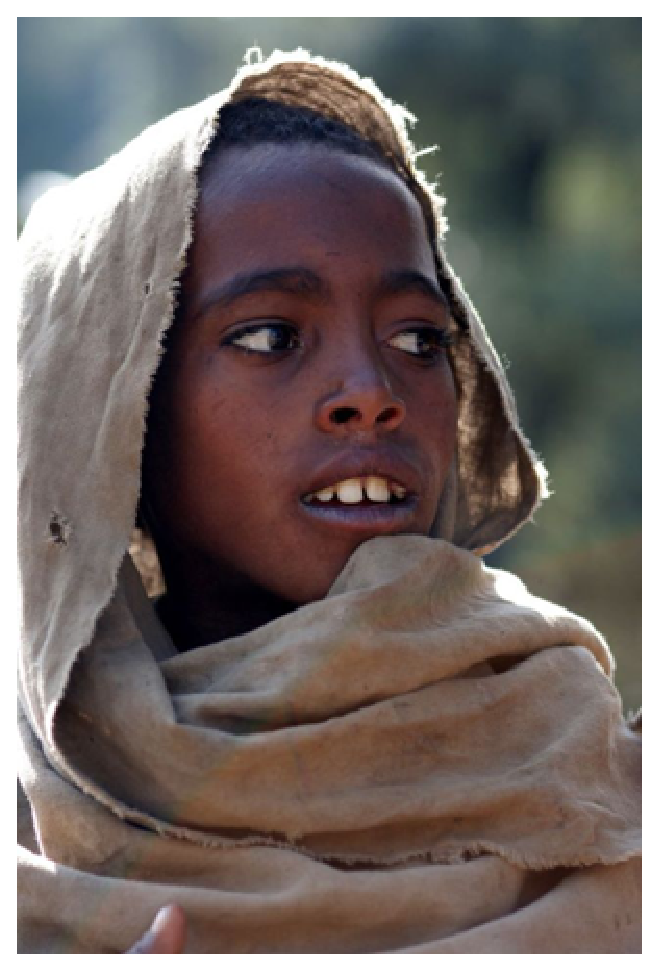
\includegraphics{etiopan.eps}
      \reflectbox{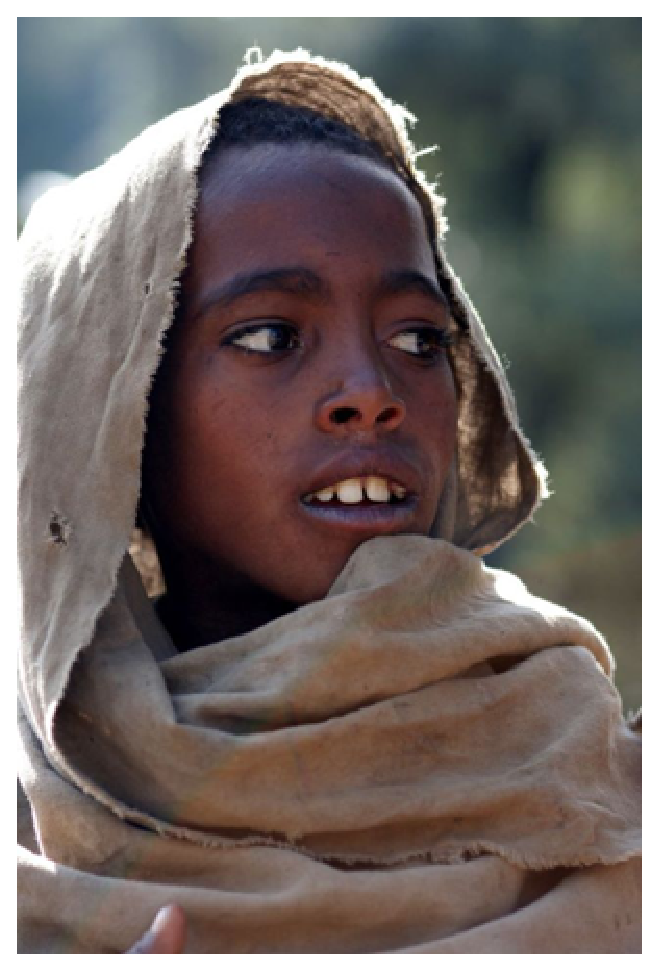
\includegraphics{etiopan.eps}}
    }
    \caption{Malý Etiopánek a~jeho bratříček}
    \label{fig:etiop}
\end{figure}
\bigskip
\footnotetext[2]{Pro nápovědu, jak zacházet s prostředím\,\, \texttt{algorithm,} můžeme zkusit tuhle stránku:\\ http://ftp.cstug.cz/pub/tex/CTAN/macros/latex/contrib/algorithms/algorithms.pdf.}
\footnotetext[3]{Pro\,\, \texttt{algorithm2e}\,\, zase tuhle: http://ftp.cstug.cz/pub/tex/CTAN/macros/latex/contrib/algorithm2e/doc/algorithm2e.pdf.}

\pagebreak
Rozdíl mezi vektorovým $\dotsc$

\begin{figure}[h]
  \centering
  \scalebox{0.4}{
  
\includegraphics{oniisan.eps}
  }
  \caption{Vektorový obrázek}
  \label{fig:onivect}
\end{figure}
\bigskip
$\dotsc$ a~bitmapovým obrázkem

\begin{figure}[h]
  \centering
  \scalebox{0.6}{
  
\includegraphics{oniisan2.eps}
  }
  \caption{Bitmapový obrázek}
  \label{fig:onibitm}
\end{figure}
\bigskip
\noindent
se projeví například při zvětšení.\par
Odkazy (nejen ty) na obrázky \ref{fig:etiop}, \ref{fig:onivect} a \ref{fig:onibitm}, na tabulky \ref{tab:price} a \ref{tab:logic} a~také na algoritmus \ref{alg:fastslam} jsou udělány pomocí křížových odkazů. Pak je ovšem potřeba zdrojový soubor přeložit dvakrát. \par
Vektorové obrázky lze vytvořit i~přímo v \LaTeX u, například pomocí prosředí\,\, \verb|picture|

\pagebreak
\begin{landscape}
  \begin{figure}[h]
    \setlength{\unitlength}{1mm}
    \centering
    \begin{picture}(200,100)
      \linethickness{1pt}
      \put(0, 0){\framebox(200,100){}}
      \linethickness{5pt}
      \put(5, 15){\line(1, 0){192}}
      \linethickness{1pt}
      \put(25,15){\line(0, 0){37}}  %lavy stlp 1.
      \put(40,15){\line(0, 0){15}}  %lavy stlp 2.
      \put(180,15){\line(0, 0){8}}  %pravy stlp 3.

      \put(40,30){\line(1, 0){40}} %schodisko podstava 2.
      \put(80,30){\line(3, -1){45}}

      \put(180,23){\line(-1, 0){79}} %shodisko podstava 1.

      \put(177,23){\line(0, 0){15}} %stlp pravo druha rada
      \put(177,38){\line(-1, 0){87}} %podlaha druhy level
      \put(90, 38){\line(0, -1){11.5}} %stlp stred 2 level

      \put(60,30){\line(-2, 3){8}}  %lava sikma hrana
      \put(52,42){\line(1,0){130}}  %podlaha 3 level
      \put(52,42){\line(0,0){5}}    %male stplce strechy
      \put(182,42){\line(0,0){5}}   %male stplce strechy
      \put(52,47){\line(1,0){130}}  %strecha

      \put(82,47){\line(0,0){11}} %strecha vycnelok stlp
      \put(82,58){\line(1,0){55}}
      \put(137,47){\line(0,0){11}}

      \put(137,49){\line(1,0){40}}
      \put(177,47){\line(0,0){2}}

      \put(25,52){\line(1,0){57}}

      \put(170,82){\circle{12}} %slnko

    \end{picture}
    \caption{Vektorový obrázek moderního bydlení vhodného pro 21. století.}
    \label{fig:tugendhat}
  \end{figure}
\end{landscape}
\end{document}
